\section{Open-AoE Toolchain}

The Open-AoE Toolchain turns synchronized egocentric video, hand geometry, camera motion, and action semantics into research assets that can be inspected, reconstructed, retargeted, and used for learning.
The released implementation, documentation, and model-integration recipes are available in the \href{https://github.com/ant-research/Open-AoE}{\raisebox{-0.15ex}{
\includegraphics[height=1.05em]{logo/github-logo.pdf}}\hspace{0.25em}Open-AoE GitHub repository}.
Each AoE sample aligns undistorted RGB, camera intrinsics and trajectories, bilateral MANO reconstruction~\cite{mano2017}, validity masks, and atomic-action annotations on one timeline.
These signals form a common evidence layer, but no single action vector is appropriate for human-motion modeling, robot control, and visual-dynamics learning at the same time.
The toolchain therefore preserves the physical meaning of the source signals and selects a representation level according to the downstream problem.

\subsection{AoE-Visualization}

AoE-Visualization is the entry point for synchronized inspection and error diagnosis.
It uses the undistorted egocentric video as the canvas, overlays MANO meshes, 21-keypoint skeletons, future wrist trajectories, and atomic actions, and presents a world-frame 3D view and timeline alongside the image.
This joint view exposes reprojection error, missing-hand intervals, SLAM drift, and semantic-boundary misalignment before a downstream model can absorb them as apparent motion regularities.
The same visual grammar is used for dataset examples and for reviewing intermediate toolchain outputs.

\subsection{AoE-Reconstruct-Retarget}

AoE-Reconstruct-Retarget connects an egocentric observation to three complementary outputs: 4D hand-object assets, robot-executable trajectories, and robotized video, as summarized in Figure~\ref{fig:reconstruct-retarget}.
The outputs are coupled: reconstruction supplies object and contact references, retargeting supplies executable motion, and robotized video places that motion back into the real visual context.

\begin{center}
    \centering
    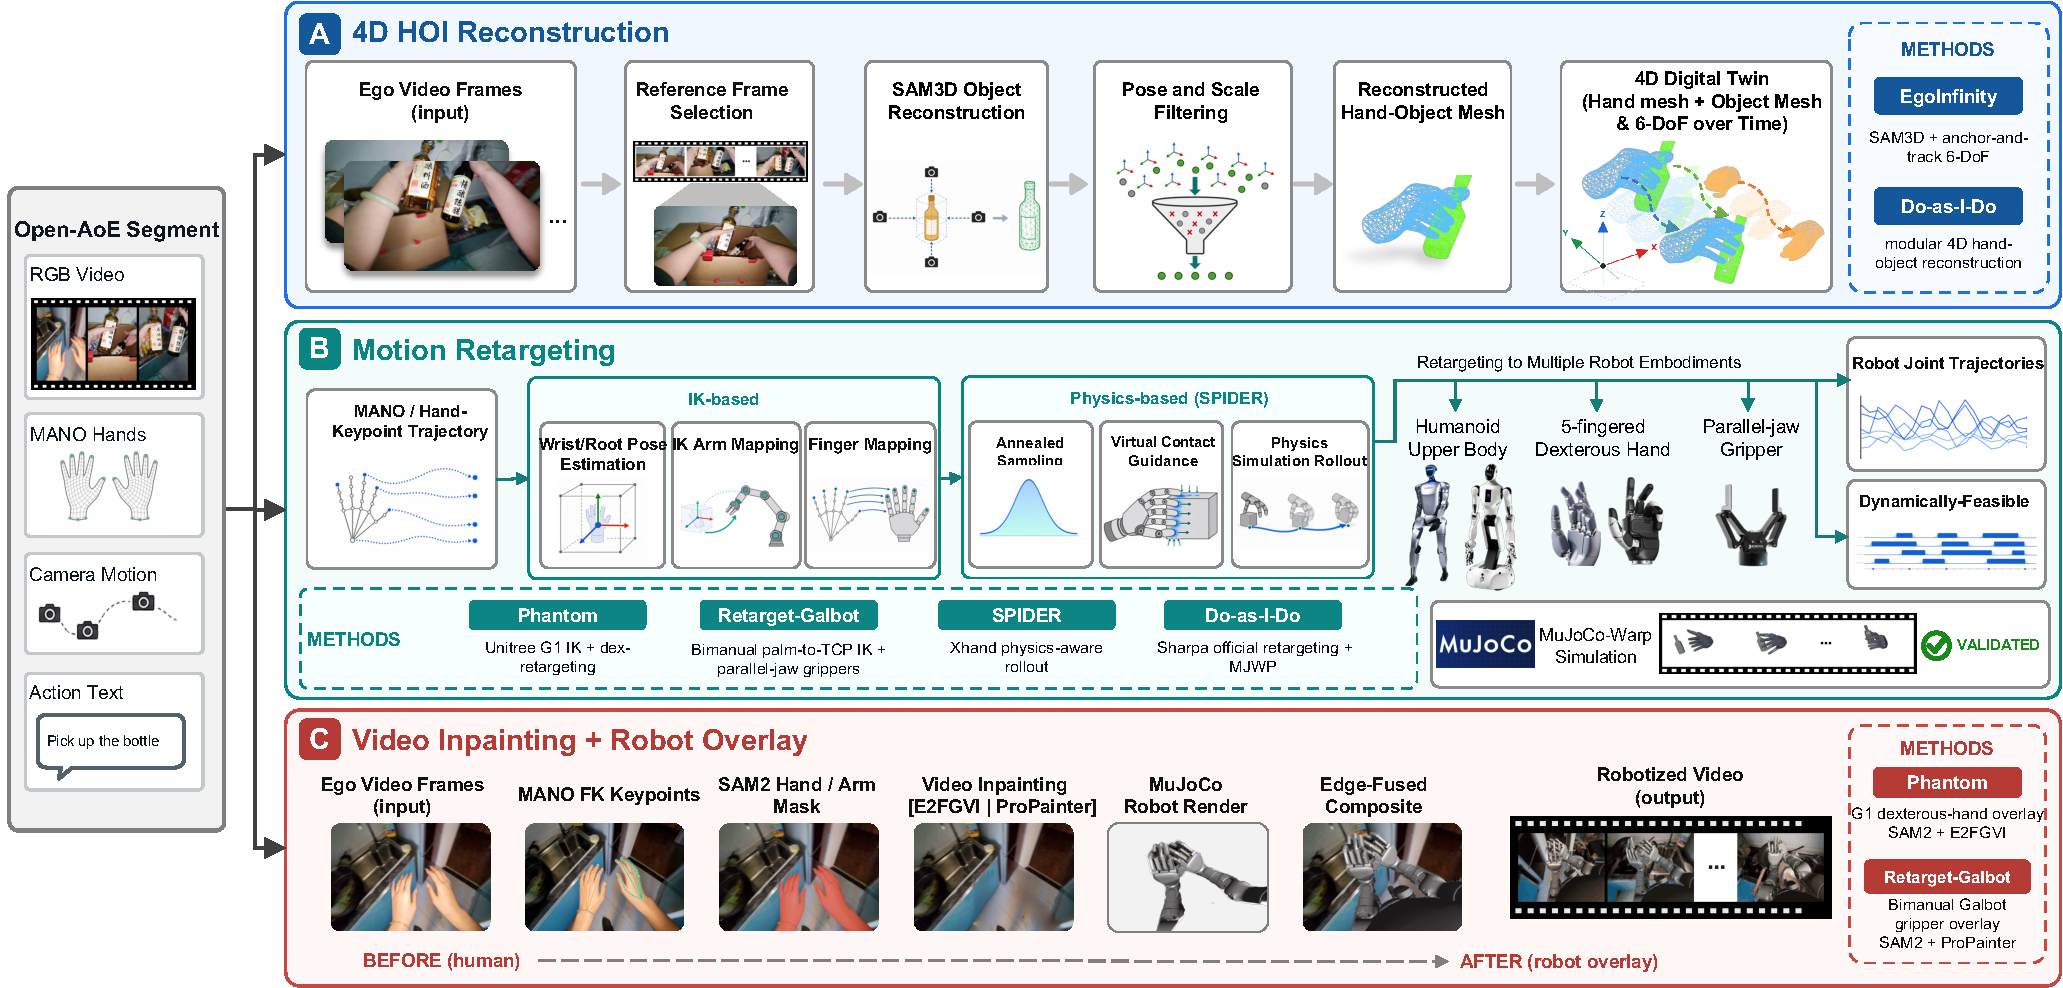
\includegraphics[width=\textwidth]{figures/fig3-reconstruct-retarget.pdf}
    \captionof{figure}{\textbf{AoE-Reconstruct-Retarget.} A smartphone-captured egocentric video is projected into 4D hand-object assets, robot-usable motion, and robotized video. The repository integrates reconstruction interfaces for EgoInfinity and Do-as-I-Do, multiple retargeting backends for G1, Galbot/Galaxea, Sharpa, and XHand, and simulation and egoview synthesis for result validation.}
    \label{fig:reconstruct-retarget}
\end{center}

\paragraph{4D hand-object reconstruction.} EgoInfinity~\cite{egoinfinity2026} and Do-as-I-Do~\cite{doasido2026} lift monocular video into time-varying hand geometry, object pose, and interaction assets.
Here, AoE contributes more than additional RGB frames: calibrated intrinsics and metric-scale camera trajectories help separate observer motion from scene motion, MANO supplies hand-scale and pose priors, and action segments delimit the temporal support of an interaction.
When combined with object 6-DoF estimates, the timing of finger approach, grasp, and release can provide contact candidates, object-tracking constraints, and priors over manipulation phases.
This allows large-scale egocentric data to convey knowledge about object affordances and hand-object coordination rather than only scene appearance.

\paragraph{Cross-embodiment retargeting.} This route asks how motion demonstrated by a human can become motion executable by a target robot.
Phantom combines arm inverse kinematics with dex-retargeting~\cite{dexretarget} to map camera-local wrist and finger motion to Unitree G1 with Dex3 or Inspire hands.
Retarget Galbot converts bimanual palm targets into Galbot/Galaxea TCP trajectories and gripper control, while Retarget Lab organizes comparable kinematic and physics-aware routes including EgoInfinity/G1, Do-as-I-Do/Sharpa, and SPIDER/XHand~\cite{spider2025}.
AoE's bilateral MANO trajectories, validity masks, and atomic-action boundaries jointly provide supervision for wrist paths, finger synergies, bimanual role assignment, and grasp timing.
Compared with isolated end-effector poses, these signals are better suited to learning cross-embodiment motion priors because they preserve the structure among reach, contact, manipulation, and release.

\paragraph{Robotized video.} This route removes the human arm and composites a simulated robot back into the original egocentric scene.
Phantom and Retarget Galbot use MANO keypoints as geometric prompts for segmentation and combine video inpainting with MuJoCo rendering to produce temporally aligned robot overlays.
Because it preserves the real environment, manipulated object, illumination, and task progression while changing the actor appearance, it can provide paired signals for human-to-robot visual-domain transfer, retargeting diagnosis, and robot-scene consistency learning.
Its value is to create aligned observations of the same interaction under different embodiments, not to treat synthesized video as a substitute for real robot execution.

\subsection{AoE-Training-Ready}

AoE-Training-Ready adapts the same synchronized source signals to model-specific action semantics rather than claiming a universal training format; Figure~\ref{fig:training-ready} summarizes this representation spectrum and its downstream model connections.
Multiple representations are necessary because human-motion learning, robot control, and video generation preserve different invariants, as summarized in Table~\ref{tab:aoe_action_representations}: human modeling benefits from finger articulation, cross-embodiment control needs end-effector or joint targets, and egocentric dynamics must account for camera self-motion.

\begin{center}
    \centering
    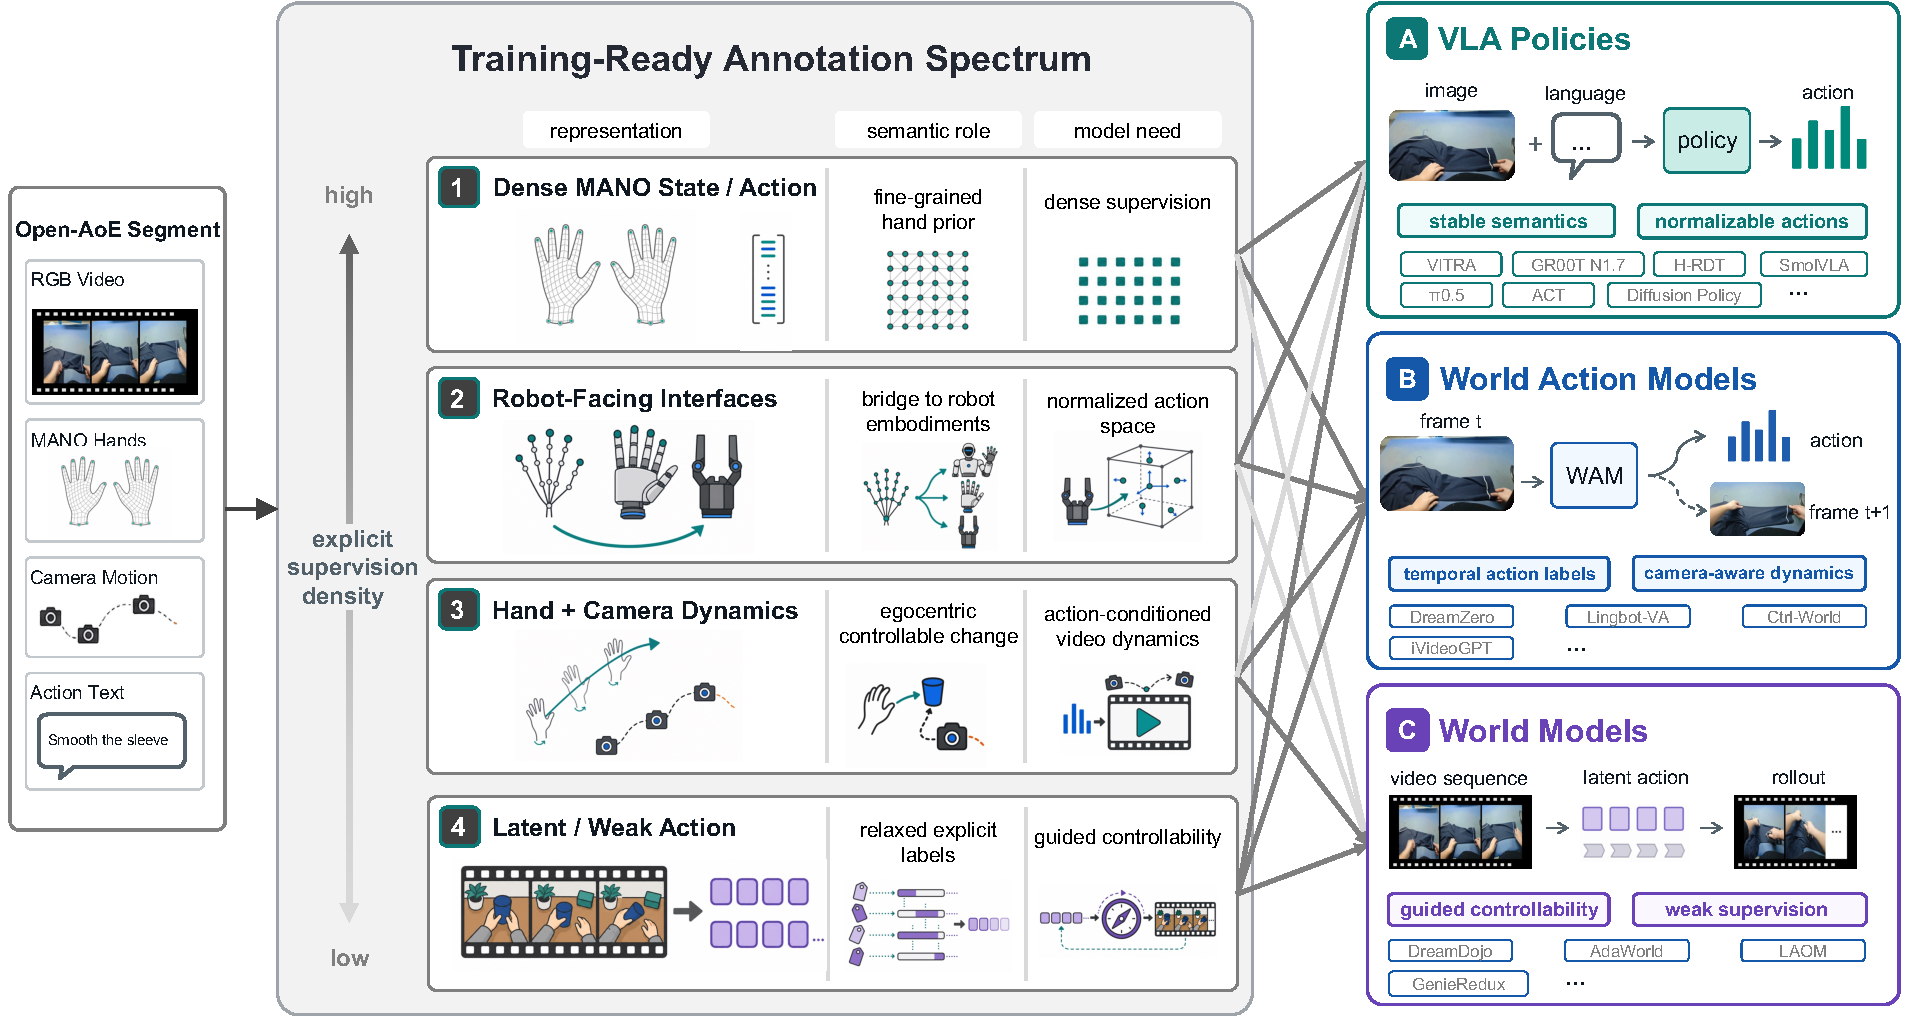
\includegraphics[width=\textwidth]{figures/fig4-training-ready.pdf}
    \captionof{figure}{\textbf{AoE-Training-Ready.} A synchronized AoE segment is projected into action representations with different supervision densities and semantic roles. Integrated recipes connect dense MANO, robot-facing, hand-plus-camera, and latent or weak action representations to Vision-Language-Action policies, World Action Models, and World Models.}
    \label{fig:training-ready}
\end{center}

For recipes that require dense hand articulation, Open-AoE concatenates two 55D per-hand vectors into a 110D representation: $2\!\times\![\mathrm{valid}(1)+\mathrm{wrist\ translation}(3)+\mathrm{wrist\ axis\mbox{-}angle}(3)+\mathrm{velocity}(3)+\mathrm{MANO\ pose}(45)]$.
Translations and finite-difference velocities are expressed in meters and meters per second in the current-frame OpenCV camera coordinates ($x$ right, $y$ down, $z$ forward), while rotations are represented in radians; because this frame moves with the wearer, the velocity contains both hand motion and camera ego-motion rather than purely inertial wrist motion.

\noindent\begin{minipage}{\textwidth}
\centering
\captionof{table}{Action representations exposed by AoE-Training-Ready. Dimensions are per-frame vectors defined by Open-AoE converters; citations identify integrated downstream methods rather than the origin of the layouts. Recipes may normalize vectors or concatenate a future horizon. The two 20D interfaces are not interchangeable.}
\label{tab:aoe_action_representations}
\footnotesize
\setlength{\tabcolsep}{3.5pt}
\begin{tabularx}{\textwidth}{>{\raggedright\arraybackslash}p{2.0cm} >{\raggedright\arraybackslash}p{4.45cm} >{\raggedright\arraybackslash}p{3.25cm} >{\raggedright\arraybackslash}X}
\toprule
Interface & Layout & Frame and units & Learning role / representative consumers \\
\midrule
110D dense MANO~\cite{mano2017} & $2\!\times\![\mathrm{valid}(1)+\mathrm{wrist}\ xyz(3)+\mathrm{wrist}\ aa(3)+\mathrm{velocity}(3)+\mathrm{MANO}(45)]$ & Current-camera frame; m, rad, m/s, binary validity & Dense hand state and next-state targets; Open-AoE adapters for LeRobot~\cite{cadene2026lerobot} and world-action recipes. \\
\midrule
48D wrist--fingertip & $2\!\times\![\mathrm{wrist}\ xyz(3)+\mathrm{rot6D}(6)+5\ \mathrm{fingertips}\ xyz(15)]$ & SLAM world frame; positions in m, rot6D unitless & Geometry-preserving target used by the Open-AoE H-RDT adapter~\cite{hrdt2025}. \\
\midrule
62D Sharpa & $L/R\ \mathrm{wrist\ EEF}(9)+L/R\ \mathrm{Sharpa\ joints}(22)$ & World-frame wrist in m + rot6D; robot joints in rad & Open-AoE GR00T N1.7 adapter~\cite{grootn172026}; actions encode wrist EEF relatively and joints absolutely. \\
\midrule
20D GR00T gripper & $L/R\ \mathrm{wrist\ EEF}(9)+L/R\ \mathrm{gripper}(1)$ & World-frame wrist in m + rot6D; gripper in $[0,1]$ & Lower-DoF Open-AoE GR00T N1.7 adapter~\cite{grootn172026}; wrist EEF is relative and gripper absolute. \\
\midrule
22D state / 20D--26D ego action & State: $2\!\times\![xyz(3)+\mathrm{rot6D}(6)+\mathrm{grip}(1)]+2\ \mathrm{valid}$; action drops validity and optionally appends camera $\Delta t(3)+\Delta r_{aa}(3)$ & Hand in current-camera frame; m and unitless rot6D/grip; camera delta in m and rad & Open-AoE adapters for SmolVLA~\cite{smolvla2025}, iVideoGPT~\cite{ivideogpt2024}, LAOM~\cite{laom2025}, and guided GenieRedux~\cite{genieredux2024}. \\
\bottomrule
\end{tabularx}
\end{minipage}

\paragraph{Policy learning and cross-embodiment control.} This route compresses egocentric human motion into targets that a policy can predict and a robot can execute.
VITRA~\cite{vitra2025}, H-RDT~\cite{hrdt2025}, GR00T N1.7~\cite{grootn172026}, SmolVLA~\cite{smolvla2025}, and LeRobot-based~\cite{cadene2026lerobot} $\pi_{0.5}$, ACT, and Diffusion Policy recipes consume dense MANO, wrist--fingertip, robot-joint, or hand-as-EEF targets according to their control abstraction.
Atomic-action language supplies task intent, framewise hand geometry supplies motion realization, bilateral trajectories supply coordination structure, and long-tailed objects and behaviors in natural scenes supply affordance and behavioral diversity.
Together, these signals support a hierarchy from observing and describing an interaction to predicting embodiment-constrained motion, without requiring robot joint labels for every human video.

\paragraph{World-action and action-conditioned video learning.} This route models how the next action or future visual state changes given the current observation and an action condition.
DreamZero~\cite{dreamzero2026}, LingBot-VA~\cite{lingbova2026}, Ctrl-World~\cite{ctrlworld2025}, and iVideoGPT~\cite{ivideogpt2024} use either dense next-hand states or compact hand-plus-camera actions to learn action prediction and visual dynamics.
Large image motion in egocentric video may arise from hand-object interaction or from motion of the head or phone; because AoE synchronizes hand and camera trajectories, these two causal sources can be represented as separate conditions or controlled variables.
This supplies direct signals for controllable visual prediction, for testing whether a model genuinely uses its action condition, and for learning action representations that are robust to a moving camera.

\paragraph{Latent-action and world-model learning.} This route discovers action variables from visual change and uses limited structured supervision to determine what those variables should represent.
GenieRedux~\cite{genieredux2024} and AdaWorld~\cite{adaworld2025} learn latent actions from videos or frame pairs, LAOM~\cite{laom2025} uses limited hand-action supervision to resist camera ego-motion as a strong distractor, and DreamDojo~\cite{dreamdojo2026} injects explicit MANO motion into its action condition.
AoE therefore contributes three forms of knowledge: scene dynamics from unlabeled video, nuisance-factor identification from camera trajectories, and controllable weak supervision from MANO motion and action segments.
The same data can move from discovering latent factors of change, to grounding those factors as hand actions, to controlling future video with explicit motion, thereby connecting unsupervised world modeling with embodied control.

Together, AoE-Visualization, AoE-Reconstruct-Retarget, and AoE-Training-Ready connect data inspection, interaction reconstruction, cross-embodiment conversion, and model learning in one traceable path.
The central design is not the number of interfaces, but the reuse of the same egocentric evidence at geometric, action, and visual-dynamics levels.
